\documentclass[runningheads]{llncs}

\usepackage[T1]{fontenc}
\usepackage[utf8]{inputenc}
\usepackage[brazilian]{babel}
\usepackage{graphicx}
\usepackage{amsmath, amssymb}
\usepackage{booktabs}
\usepackage{subcaption}
\usepackage{multirow}
\usepackage{placeins}

\graphicspath{{figs/}}

\emergencystretch=1.5em

\begin{document}

\title{Data Drift in a Seq2Seq Model for SSL Robot Trajectory Prediction}
\titlerunning{Data Drift in Seq2Seq SSL Trajectory Prediction}

\author{Ivan G. Yamasaki\inst{1}\orcidID{0009-0000-4776-134X} \and
Marcos R. O. A. M\'aximo\inst{1}\orcidID{0000-0003-2944-4476} \and
Paulo M. Tasinaffo\inst{1}\orcidID{0000-0001-7069-8430}}
%
\authorrunning{I. Yamasaki et al.}
%
\institute{Aeronautics Institute of Technology, S\~ao Jos\'e dos Campos, Brazil}
%
\maketitle

\begin{abstract}
Este artigo analisa \textit{data drift} em um modelo \textit{sequence-to-sequence} (seq2seq) de predi\c{c}\~ao de trajet\'orias na RoboCup Small Size League (SSL), treinado com dados de 2019 e avaliado nas temporadas de 2021 a 2025. O erro absoluto (\textit{Average Displacement Error}, ADE) cresce de forma persistente ap\'os o treino~--- excessos de at\'e $+0{,}73$\,mm em 2022--2025, al\'em do salto de $+3{,}05$\,mm na edi\c{c}\~ao virtual de 2021 (horizonte $30{\to}15$)~---, enquanto o benchmark de Kalman degrada ainda mais~--- a vantagem relativa do modelo neural aumenta sob drift. A origem da degrada\c{c}\~ao \'e quantificada por \textit{importance weighting} via LSIF, com robustez verificada por truncamento de pesos e pela transforma\c{c}\~ao de raz\~ao relativa, e validada por um \textit{classifier two-sample test} independente: 59--72\,\% do excesso de ADE \'e explic\'avel por \textit{covariate shift}, com a acelera\c{c}\~ao de cauda (\texttt{accel\_p99}) como dimens\~ao dominante.

Na adapta\c{c}\~ao~--- restrita a 2019 (regime antigo) e 2022--2025 (dados novos), com a edi\c{c}\~ao virtual de 2021 exclu\'ida como \emph{outlier}~---, o \textit{catastrophic forgetting} cai de 0{,}82 para 0{,}46 (\texttt{cat\_ratio}) com ajuste conservador; um sweep de $\lambda$ ao longo de 8 ordens de grandeza mostra que a prote\c{c}\~ao vem da taxa de aprendizado baixa, n\~ao da regulariza\c{c}\~ao EWC. Por fim, a calibra\c{c}\~ao de detectores online sobre o stream de 288\,k trajet\'orias, validada por holdout 2-fold por jogos, produz um detector operacional (ADWIN sobre o erro, com pr\'e-processamento z-robusto): $\mathrm{FAR}_{2019}$ de $0{,}04$--$0{,}13$/1k fora da amostra, cobertura de 9/10 anos-fold e lat\^encia de $0{,}2$--$1{,}5$ jogo. O vetor dominante do drift fornece ainda um canal de vigil\^ancia \emph{model-free} (\texttt{accel\_p95}) que antecipa o alarme de erro em 8/10 anos-fold, e a conjun\c{c}\~ao erro$\wedge$acelera\c{c}\~ao zera os falsos alarmes observados.
\keywords{predi\c{c}\~ao de trajet\'orias \and seq2seq \and data drift \and detec\c{c}\~ao de drift \and RoboCup SSL \and Kalman}
\end{abstract}

\section{Introdu\c{c}\~ao}

Predi\c{c}\~ao de trajet\'orias \'e uma tarefa central em sistemas aut\^onomos sujeitos a din\^amica r\'apida. Na RoboCup SSL, prever a movimenta\c{c}\~ao futura dos rob\^os auxilia planejamento, posicionamento e tomada de decis\~ao em tempo real.

O filtro de Kalman~\cite{kalman} \'e o benchmark tradicional nesse problema por ser simples e barato, mas depende de hip\'oteses cinem\'aticas restritivas~--- din\^amica suave, bem descrita por modelos lineares locais. Modelos seq2seq capturam depend\^encias temporais mais ricas e aprendem padr\~oes de a\c{c}\~ao futura diretamente dos dados. Por\'em, melhor desempenho em um per\'iodo espec\'ifico n\~ao garante robustez temporal: se a din\^amica do jogo muda entre temporadas, um modelo treinado em dados antigos degrada. Esse \'e o problema de \textit{data drift} analisado aqui.

O ponto de partida \'e o modelo seq2seq de Steuernagel e M\'aximo~\cite{seq2seq} para predi\c{c}\~ao de trajet\'orias na SSL. A contribui\c{c}\~ao deste artigo n\~ao \'e uma nova arquitetura, mas a reavalia\c{c}\~ao temporal desse modelo de refer\^encia, organizada em quatro perguntas:

\begin{enumerate}
    \item como o erro evolui ao longo das temporadas, em dois horizontes de predi\c{c}\~ao, e como essa evolu\c{c}\~ao se compara ao benchmark de Kalman;
    \item que fra\c{c}\~ao da degrada\c{c}\~ao \'e explic\'avel por \textit{covariate shift} (mudan\c{c}a na distribui\c{c}\~ao de entrada) e qual dimens\~ao cinem\'atica a domina;
    \item se a adapta\c{c}\~ao leve (fine-tuning seletivo, EWC~\cite{kirkpatrick2017}) recupera desempenho sem esquecimento catastr\'ofico;
    \item se \'e poss\'ivel operar um detector online de drift com taxa de falsos alarmes, cobertura e lat\^encia adequadas para acionar retreino.
\end{enumerate}

\section{Trabalhos relacionados}

\paragraph{Predi\c{c}\~ao de trajet\'orias.}
A linha de pesquisa evoluiu do \textit{social pooling} entre LSTMs vizinhas (Social-LSTM~\cite{alahi2016}) para grafos din\^amicos com vari\'aveis latentes multimodais (Trajectron++~\cite{salzmann2020}), Transformers \textit{agent-aware} (AgentFormer~\cite{yuan2021}) e modelos de difus\~ao (MID~\cite{gu2022}). No dom\'inio SSL, Steuernagel e M\'aximo~\cite{seq2seq} aplicaram a arquitetura seq2seq com aten\c{c}\~ao e os mesmos horizontes aqui estudados~--- \'e o baseline direto deste trabalho. Essa literatura avalia modelos em recortes fixos; a estabilidade \emph{temporal} entre temporadas, foco deste artigo, permanece pouco explorada.

\paragraph{Drift e detec\c{c}\~ao online.}
Gama et al.~\cite{gama2014} distinguem \textit{virtual drift} (mudan\c{c}a em $p(x)$) de \textit{real drift} (mudan\c{c}a em $p(y|x)$), e os detectores dividem-se entre \textit{error-based}~--- ADWIN~\cite{adwin}, Page-Hinkley~\cite{page_hinkley}~--- e \textit{data-based}, como KSWIN~\cite{kswin}. Lu et al.~\cite{lu2019} apontam a calibra\c{c}\~ao da taxa de falsos alarmes como requisito central de confiabilidade~--- exatamente a lacuna que a Se\c{c}\~ao~\ref{sec:deteccao} fecha por busca em grade sobre o stream real, complementada por valida\c{c}\~ao de lat\^encia e de robustez \`a depend\^encia serial.

\paragraph{Covariate shift.}
A estima\c{c}\~ao direta da raz\~ao de densidades via LSIF/KLIEP~\cite{kliep,kanamori2009,sugiyama_book} permite corrigir covariate shift sem retreinar; o RuLSIF~\cite{yamada2013} \'e a variante de raz\~ao relativa com pesos limitados, e o \textit{classifier two-sample test}~\cite{lopezpaz2017} oferece um detector de shift independente de forma. Este artigo usa o LSIF como estimador principal, verifica sua robustez diretamente~--- truncamento de pesos e transforma\c{c}\~ao de raz\~ao relativa (Se\c{c}\~ao~\ref{sec:iw})~--- e emprega o classifier como valida\c{c}\~ao independente.

\section{Metodologia}
\label{sec:metodologia}

\paragraph{Dados.}
S\~ao usados registros oficiais de partidas dos campeonatos mundiais de 2019 a 2025 (2020 exclu\'ido por aus\^encia de campeonato presencial): 6 jogos por ano, 36 jogos no total, capturados a 60\,Hz, todos da Divis\~ao A. O ano de 2021 corresponde \`a edi\c{c}\~ao p\'os-pand\^emica realizada virtualmente (partidas em simula\c{c}\~ao) e \'e mantido nas an\'alises descritivas por representar o salto de distribui\c{c}\~ao mais severo ($+3{,}05$\,mm de excesso de ADE)~--- com a ressalva de que parte desse salto pode refletir a lacuna simula\c{c}\~ao--real, e n\~ao apenas drift org\^anico da liga; por isso as an\'alises por ano o sinalizam separadamente. Por essa mesma raz\~ao~--- por ser uma edi\c{c}\~ao \emph{virtual}, com distribui\c{c}\~ao de vari\'aveis cinem\'aticas fora do padr\~ao das temporadas presenciais e o maior deslocamento de covariate shift do per\'iodo~---, 2021 \'e tratado como \emph{outlier} e \textbf{exclu\'ido da an\'alise de adapta\c{c}\~ao} (Se\c{c}\~ao~\ref{sec:adaptacao}): consolidar o modelo tomando como refer\^encia uma temporada anômala e simulada contaminaria o regime antigo com uma distribui\c{c}\~ao que n\~ao representa o comportamento real da liga. Nessa an\'alise, portanto, o regime antigo \'e apenas 2019 (o baseline presencial de treino) e os dados novos s\~ao 2022--2025. Como a composi\c{c}\~ao da liga \'e constante nos dados, o excesso observado n\~ao \'e atribu\'ivel a mudan\c{c}a de divis\~ao. Para as an\'alises por trajet\'oria, amostram-se 8\,000 janelas por jogo, formando um stream temporalmente ordenado de 288\,000 trajet\'orias (48\,000 por ano). O baseline de 2019 usa \emph{todos} os 6 jogos do ano: um \emph{sweep} de sensibilidade mostra que, com apenas 1 jogo de refer\^encia, $\mathrm{ADE}_{2019}$ varia de 4{,}53 a 6{,}20\,mm~--- o suficiente para inverter o sinal do excesso em 4 dos 5 anos~--- o que torna o baseline completo uma decis\~ao metodol\'ogica cr\'itica.\footnote{C\'odigo do pipeline e dados processados dispon\'iveis mediante solicita\c{c}\~ao aos autores.}

\paragraph{Etapas.}
A an\'alise tem cinco etapas: (i)~replica\c{c}\~ao do modelo de refer\^encia~\cite{seq2seq} (descrito na Se\c{c}\~ao~\ref{sec:arquitetura}); (ii)~avalia\c{c}\~ao anual do erro e compara\c{c}\~ao com o benchmark de Kalman; (iii)~quantifica\c{c}\~ao do \textit{covariate shift} por \textit{importance weighting} (LSIF), com verifica\c{c}\~oes de robustez e valida\c{c}\~ao por \textit{classifier two-sample test}; (iv)~experimentos de adapta\c{c}\~ao (fine-tuning, EWC, replay e sele\c{c}\~ao dirigida pelo diagn\'ostico); (v)~calibra\c{c}\~ao sistem\'atica de detectores online sobre o stream de ADE, com valida\c{c}\~ao de lat\^encia, de robustez da taxa de falsos alarmes e de ensembles.

Na replica\c{c}\~ao, a entrada de cada passo temporal \'e composta por seis vari\'aveis normalizadas: posi\c{c}\~ao \(x,y\), velocidade \(v_x,v_y\) e orienta\c{c}\~ao \(\sin(\psi), \cos(\psi)\). O treinamento usa valida\c{c}\~ao fixa de 10\,\%, \textit{batch size} 1024, otimizador Adam~\cite{adam} com taxa de aprendizado inicial $10^{-3}$ (\textit{clipnorm} 1{,}0), \textit{early stopping} com paci\^encia 8 e redu\c{c}\~ao adaptativa da taxa de aprendizado~--- detalhes mantidos fixos para que a compara\c{c}\~ao temporal reflita mudan\c{c}as nos dados, n\~ao no ajuste.

A m\'etrica principal \'e o ADE. Para \(N\) trajet\'orias e horizonte \(H\),
\begin{equation}\label{eq:ade}
\mathrm{ADE} = \frac{1}{NH} \sum_{i=1}^{N}\sum_{t=1}^{H} \left\lVert \hat{p}_{i,t} - p_{i,t} \right\rVert_2,
\end{equation}
em que \(\hat{p}_{i,t}\) \'e a posi\c{c}\~ao prevista e \(p_{i,t}\) a real. As an\'alises descritivas reportam os horizontes \(30 \rightarrow 15\) e \(60 \rightarrow 30\); as an\'alises de mecanismo e detec\c{c}\~ao usam o horizonte \(30 \rightarrow 15\).

\section{Arquitetura do modelo}
\label{sec:arquitetura}

O modelo segue a arquitetura \textit{encoder-decoder} de Steuernagel e M\'aximo~\cite{seq2seq}: encoder LSTM com 128 unidades, aten\c{c}\~ao aditiva de Bahdanau et al.~\cite{bahdanau} e decoder LSTM auto-regressivo, sem \textit{teacher forcing}~--- a primeira entrada do decoder \'e a \'ultima velocidade observada e os passos seguintes reutilizam as sa\'idas previstas. A cada passo do decoder, a aten\c{c}\~ao pondera os estados ocultos do encoder por \textit{softmax} sobre escores aditivos, produzindo o vetor de contexto que alimenta a predi\c{c}\~ao.

O treinamento minimiza a perda combinada
\begin{equation}\label{eq:loss}
\mathcal{L} = 100 \cdot (\mathrm{MSE} + \mathrm{MAE}).
\end{equation}
O fator 100 \'e um reescalonamento num\'erico herdado da implementa\c{c}\~ao de refer\^encia~\cite{seq2seq}. Um detalhe relevante para a an\'alise de drift: o alvo \'e parametrizado no espa\c{c}o de velocidades incrementais normalizadas (\texttt{dv}), e a trajet\'oria futura em posi\c{c}\~ao \'e reconstru\'ida a partir do \'ultimo estado observado. O modelo prev\^e, portanto, uma din\^amica futura acumulada no espa\c{c}o de estados~--- o que o torna diretamente sens\'ivel a mudan\c{c}as na distribui\c{c}\~ao de velocidades e acelera\c{c}\~oes.

\paragraph{Benchmark de Kalman.}
O comparador cinem\'atico \'e o preditor de velocidade constante correspondente ao regime estacion\'ario de um filtro de Kalman~\cite{kalman} com modelo CV: no espa\c{c}o \texttt{dv}, os incrementos de velocidade previstos s\~ao nulos~--- a velocidade \'e mantida no \'ultimo valor observado e a posi\c{c}\~ao \'e extrapolada linearmente. \'E determin\'istico, livre de par\^ametros ajust\'aveis e id\^entico em todos os anos, o que o torna uma refer\^encia fixa: qualquer degrada\c{c}\~ao sua reflete exclusivamente mudan\c{c}a no comportamento dos rob\^os.

\section{Degrada\c{c}\~ao temporal do erro}
\label{sec:degradacao}

A Figura~\ref{fig:degradacao} consolida os tr\^es fatos descritivos centrais.

\begin{figure}[t]
    \centering
    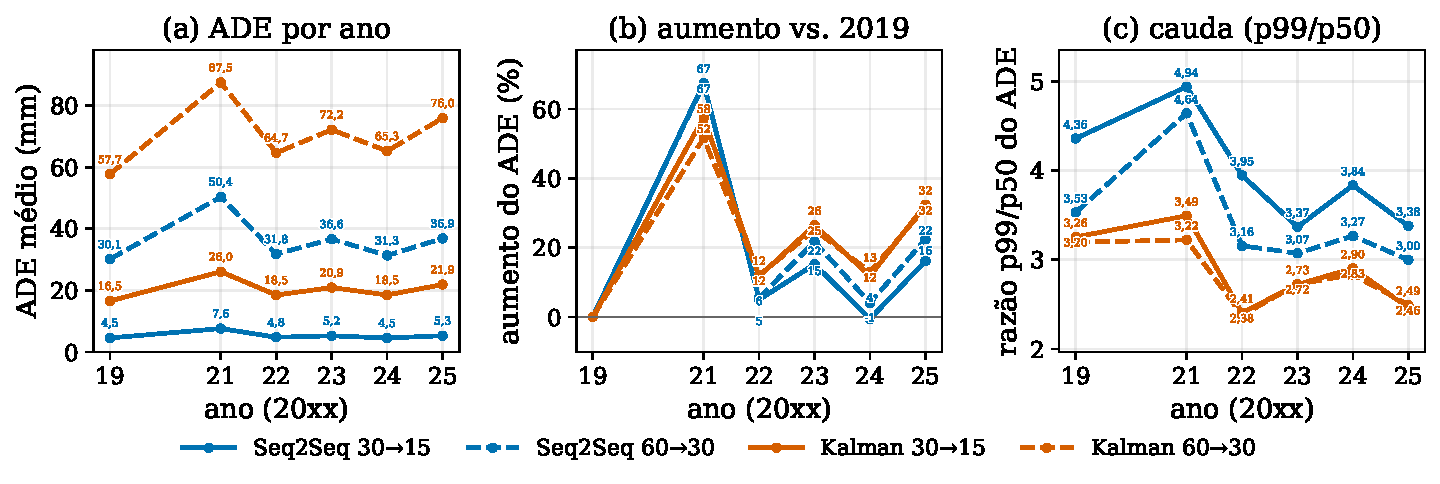
\includegraphics[width=\linewidth]{fig_degradacao_pt}
    \caption{Degrada\c{c}\~ao temporal consolidada (cor = modelo; tra\c{c}o = horizonte). (a)~ADE m\'edio por ano: o seq2seq degrada ap\'os 2019, com excesso crescente em 2022--2025 e salto adicional na edi\c{c}\~ao virtual de 2021; permanece muito abaixo do Kalman. (b)~Aumento percentual do ADE em rela\c{c}\~ao a 2019 por modelo e horizonte. (c)~Raz\~ao $\mathrm{p99}/\mathrm{p50}$ do ADE por trajet\'oria: o salto de 2021 \'e de cauda ($4{,}36 \to 4{,}94$); em 2022--2025 a raz\~ao fica abaixo do baseline ($3{,}4$--$4{,}0$), com o p50 subindo ${\approx}25\,\%$ at\'e 2025 e o p99 est\'avel~--- a degrada\c{c}\~ao gradual ocorre no corpo da distribui\c{c}\~ao.}
    \label{fig:degradacao}
\end{figure}

\textbf{(a) O seq2seq degrada fora da distribui\c{c}\~ao de treino.} O ADE cresce em todos os anos p\'os-2019, com tend\^encia de excesso crescente em 2022--2025 ($+0{,}23$\,mm em 2022 $\to$ $+0{,}73$\,mm em 2025, com 2024 pr\'oximo de zero, no horizonte $30{\to}15$). O ano de 2021 destoa ($+67\,\%$) porque acumula um fator de erro adicional: a edi\c{c}\~ao foi realizada em simula\c{c}\~ao (Se\c{c}\~ao~\ref{sec:metodologia}). O padr\~ao se repete nos dois horizontes.

\textbf{(b) O Kalman degrada mais.} O crescimento percentual do erro do Kalman supera o do seq2seq em praticamente todos os anos. A leitura correta n\~ao \'e que o seq2seq esteja est\'avel~--- seu erro absoluto tamb\'em cresce~--- mas que o benchmark cinem\'atico \'e ainda mais sens\'ivel \`a mudan\c{c}a de regime: a vantagem comparativa do modelo neural \emph{aumenta} sob drift.

\textbf{(c) O regime novo entra pela cauda e depois se generaliza.} A raz\~ao $\mathrm{p99}/\mathrm{p50}$ do seq2seq sobe apenas no salto de 2021 ($4{,}36 \to 4{,}94$), quando o modelo falha desproporcionalmente em uma cauda de trajet\'orias. Nos anos seguintes a raz\~ao cai abaixo do baseline ($3{,}4$--$4{,}0$): o p50 sobe ${\approx}25\,\%$ at\'e 2025 enquanto o p99 permanece est\'avel~--- o comportamento que era raro torna-se comum, e a degrada\c{c}\~ao gradual ocorre no corpo da distribui\c{c}\~ao. Isso \'e coerente com o covariate shift dominado por acelera\c{c}\~ao de cauda (\texttt{accel\_p99}, Se\c{c}\~ao~\ref{sec:iw}): a din\^amica agressiva que definia a cauda incorpora-se \`a distribui\c{c}\~ao t\'ipica das temporadas seguintes.

\section{Drift nas vari\'aveis cinem\'aticas}
\label{sec:cinematica}

A Figura~\ref{fig:cinematica} examina se a degrada\c{c}\~ao acompanha mudan\c{c}as mensur\'aveis na distribui\c{c}\~ao das vari\'aveis de velocidade, acelera\c{c}\~ao e giro, medidas por duas estat\'isticas independentes contra o baseline de 2019: Kolmogorov--Smirnov (KS) e dist\^ancia de Wasserstein (WD).

\begin{figure}[t]
    \centering
    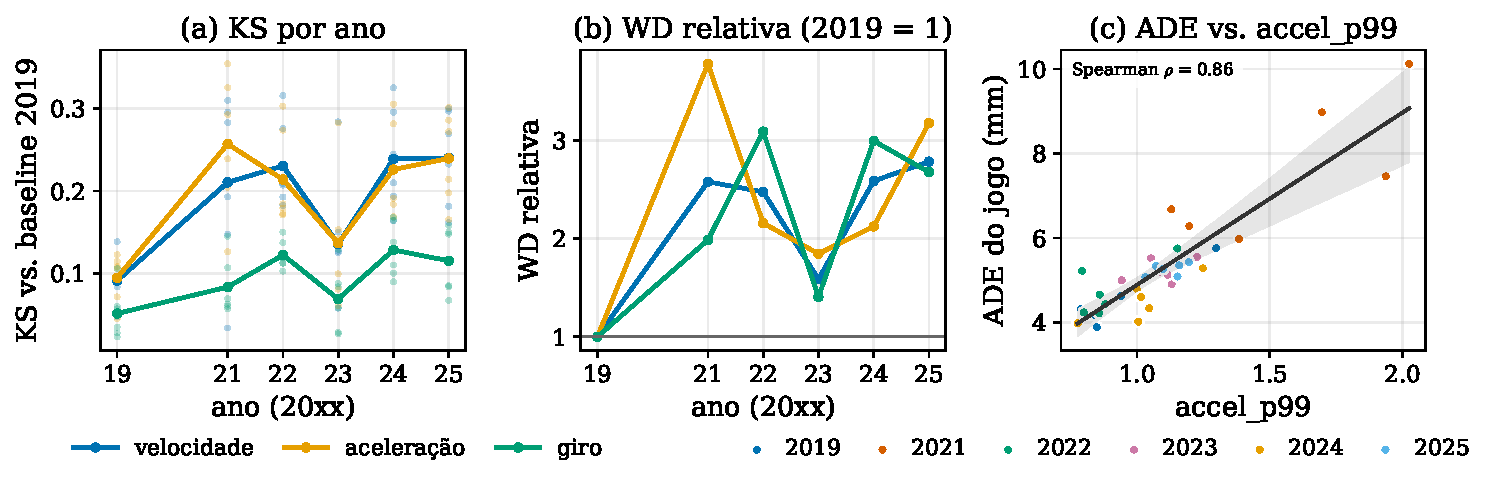
\includegraphics[width=\linewidth]{fig_drift_cinematico_pt}
    \caption{Drift cinem\'atico consolidado. (a)~Estat\'istica KS por ano contra o baseline 2019 (linhas = m\'edia anual; pontos = jogos): velocidade e acelera\c{c}\~ao mudam mais que giro. (b)~Wasserstein indexada ao n\'ivel de 2019 (=1): as duas fam\'ilias de m\'etricas concordam qualitativamente; a acelera\c{c}\~ao apresenta o maior deslocamento distribucional. (c)~ADE m\'edio por jogo contra \texttt{accel\_p99} do jogo (reta de regress\~ao com IC\,95\,\% bootstrap): a associa\c{c}\~ao \'e forte (Spearman $\rho = 0{,}86$) e consistente entre anos.}
    \label{fig:cinematica}
\end{figure}

Velocidade e acelera\c{c}\~ao mudam de forma clara e persistente nos anos p\'os-2019, com KS e WD concordando qualitativamente; o giro muda menos. No n\'ivel de jogo, o ADE cresce quase monotonicamente com a acelera\c{c}\~ao de cauda do jogo (\texttt{accel\_p99}, painel~c)~--- partidas mais agressivas s\~ao exatamente aquelas em que o modelo mais erra, independentemente do ano.

A Figura~\ref{fig:corr_spearman} sintetiza as associa\c{c}\~oes: as correla\c{c}\~oes mais fortes com o ADE do seq2seq envolvem as features de acelera\c{c}\~ao de cauda (\texttt{accel\_p90}, \texttt{accel\_p99}), antecipando o resultado por feature da decomposi\c{c}\~ao por \textit{importance weighting} (Tabela~\ref{tab:iw_feat}). Essas associa\c{c}\~oes s\~ao descritivas~--- a quantifica\c{c}\~ao causal da fra\c{c}\~ao do erro atribu\'ivel ao covariate shift \'e feita na Se\c{c}\~ao~\ref{sec:iw}.

\begin{figure}[t]
    \centering
    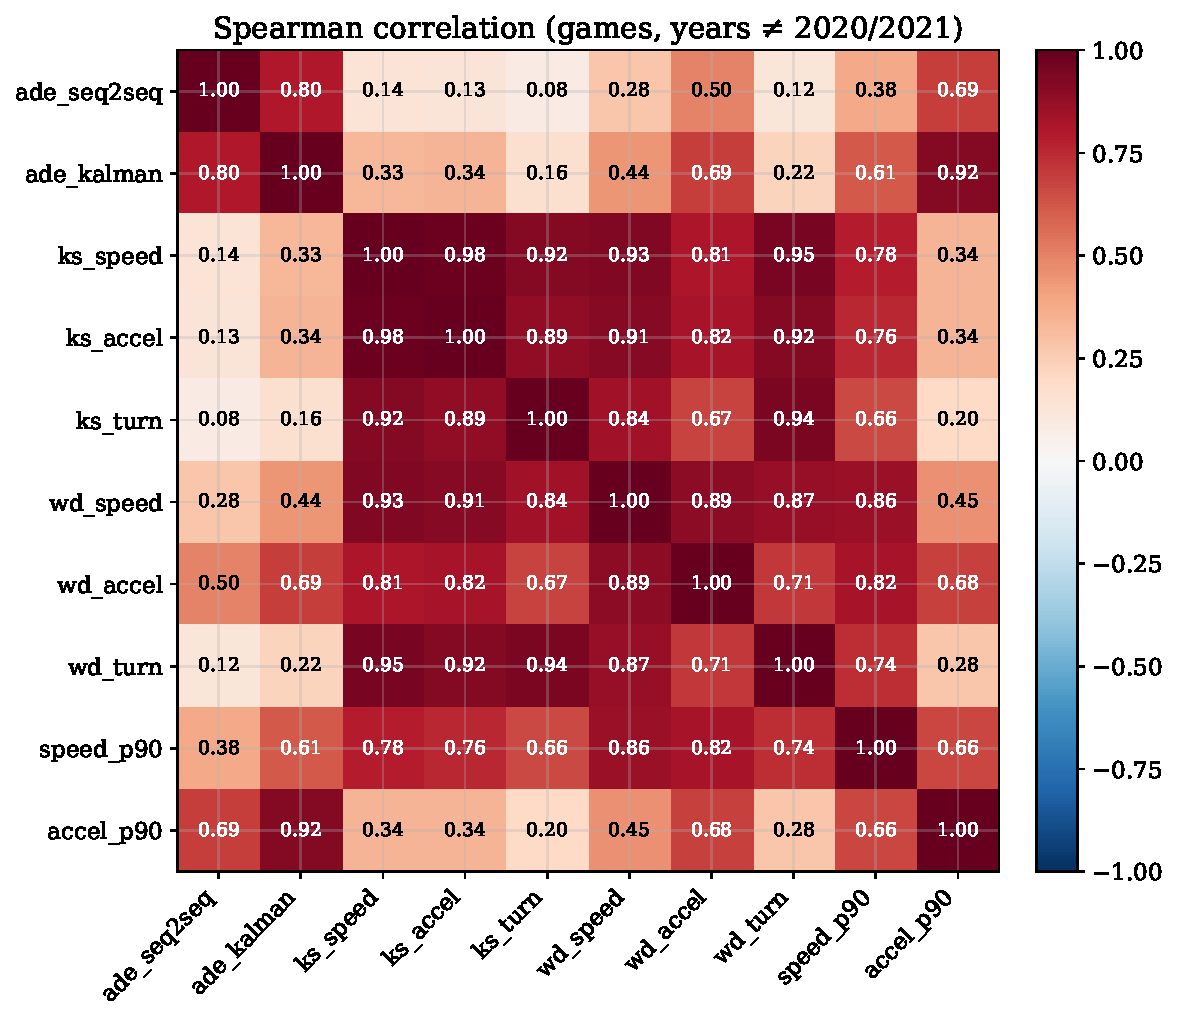
\includegraphics[width=0.72\linewidth]{4d_corr_spearman_pt}
    \caption{Correla\c{c}\~ao de Spearman entre o ADE por jogo e as features de drift (anos $\neq$ 2020/2021).}
    \label{fig:corr_spearman}
\end{figure}

\section{Quantifica\c{c}\~ao do drift via importance weighting}
\label{sec:iw}

\paragraph{Decomposi\c{c}\~ao covariate vs.\ concept drift.}
A distribui\c{c}\~ao conjunta fatoriza-se como $p(x,y) = p(y|x)\,p(x)$~\cite{gama2014}. O \emph{covariate shift} altera apenas $p(x)$ e pode ser corrigido por repondera\c{c}\~ao dos exemplos antigos, sem retreinar; o \emph{concept drift} altera $p(y|x)$ e exige novos dados rotulados. Distinguir as componentes \'e o que justifica o \textit{importance weighting} (IW): se o drift for majoritariamente covariate, a corre\c{c}\~ao \'e barata.

\paragraph{LSIF e ADE ponderado.}
O LSIF (\emph{Least-Squares Importance Fitting})~\cite{kliep,kanamori2009,sugiyama_book} estima diretamente a raz\~ao de densidades $\hat{w}(x) = p_{\text{alvo}}(x)/p_{2019}(x)$ como combina\c{c}\~ao de kernels gaussianos. O vetor $x \in \mathbb{R}^{8}$ re\'une as features cinem\'aticas da janela observada de cada trajet\'oria~--- m\'edia, p90 e p99 da velocidade e da acelera\c{c}\~ao, e m\'edia e p90 do giro~---, com corte no percentil 99{,}5 do pool (estabiliza a cauda) e transforma\c{c}\~ao $\log(1+\cdot)$:
\begin{equation}\label{eq:lsif}
\min_{\boldsymbol\alpha \geq 0}\;
\tfrac{1}{2}\,\mathbb{E}_{p_{2019}}[\hat{w}(x)^2] -
\mathbb{E}_{p_{\text{alvo}}}[\hat{w}(x)] + \lambda\|\boldsymbol\alpha\|^2.
\end{equation}
A estabilidade \'e diagnosticada pelo \emph{Effective Sample Size} (ESS),
definido como $(\sum_i \hat{w}_i)^2/(n\sum_i \hat{w}_i^2)$, com regra
pr\'atica $\mathrm{ESS} > 0{,}5$~\cite{sugiyama_book}. A partir dos pesos,
definem-se o ADE ponderado e a fra\c{c}\~ao recuperada do excesso:
\begin{equation}\label{eq:recovery}
\mathrm{ADE}_{\mathrm{IW}}(y) =
    \frac{\sum_i \hat{w}(x_i)\,e_i}{\sum_i \hat{w}(x_i)}, \qquad
\mathrm{recovery}(y) =
    \frac{\mathrm{ADE}_y - \mathrm{ADE}_{\mathrm{IW}}(y)}
         {\mathrm{ADE}_y - \mathrm{ADE}_{2019}} \times 100\,\%.
\end{equation}
Recovery de 100\,\% indicaria drift puramente covariate; 0\,\%, concept drift puro.

\paragraph{Robustez do estimador e valida\c{c}\~ao independente.}
A leitura quantitativa exige confian\c{c}a no comportamento dos pesos, sobretudo sob caudas pesadas (\texttt{accel\_p99}). Tr\^es verifica\c{c}\~oes diretas sustentam o LSIF. (i)~\emph{Pesos limitados}: $\max_i \hat{w}_i \in [2{,}9;\,4{,}4]$ em todos os anos; o ESS de $0{,}58$--$0{,}73$ reflete a massa de pesos ${\approx}\,0$ atribu\'ida ao regime novo~--- o mecanismo correto de reconstru\c{c}\~ao de 2019~---, e n\~ao pesos extremos (o top-1\,\% das trajet\'orias carrega apenas 3--4\,\% da massa). (ii)~\emph{Insensibilidade a truncamento}: um sweep de cap $c \in \{1{,}5,\ldots,50\}$ mostra que a recovery satura em $c \approx 3$--$5$. (iii)~\emph{Insensibilidade \`a raz\~ao relativa}: aplicar aos pesos a transforma\c{c}\~ao $\hat{w}/(\alpha\hat{w}+1-\alpha)$ do RuLSIF~\cite{yamada2013} ($\alpha\,{=}\,0{,}1$) mant\'em a recovery em 59--65\,\%. O RuLSIF ajustado diretamente foi testado e descartado: nesta configura\c{c}\~ao produz pesos quase uniformes ($\mathrm{ESS} \geq 0{,}94$) e sub-responde (recovery 9--23\,\%)~--- artefato da regulariza\c{c}\~ao do ajuste, n\~ao do estimando, como as verifica\c{c}\~oes (ii) e (iii) demonstram. A valida\c{c}\~ao independente \'e o \textit{classifier two-sample test}~\cite{lopezpaz2017}: regress\~ao log\'istica que separa 2019 do ano-alvo, com cobertura $\mathrm{cov} = \mathrm{clip}(2\,(\mathrm{AUC}-0{,}5)\cdot 100,\,0,\,100)$. Os intervalos usam \emph{block bootstrap} com bloco = jogo e denominador fixado no excesso observado~--- a raz\~ao por r\'eplica degenera com 6 blocos quando o excesso \'e pequeno. A Tabela~\ref{tab:iw_decomp} consolida.

\begin{table}[t]
\centering
\caption{Decomposi\c{c}\~ao IW (LSIF) com block bootstrap por jogo
         ($n_{\text{boot}}\,{=}\,2\,000$; $n_{\text{blocos}}\,{=}\,6$ jogos/ano);
         ICs de recovery com denominador fixado no excesso observado.
         Baseline: $\mathrm{ADE}_{2019} = 4{,}53$\,mm; excesso $=$
         $\mathrm{ADE}_y - \mathrm{ADE}_{2019}$. $\mathrm{ADE}_{\mathrm{IW}}$
         \'e o ADE do ano reponderado para a distribui\c{c}\~ao de 2019;
         corr.\ = $\mathrm{ADE}_y - \mathrm{ADE}_{\mathrm{IW}}$: o limite
         inferior \'e positivo em todos os anos com excesso.
         $\mathrm{ESS} \in [0{,}58;\,0{,}73]$. 2024 tem excesso negativo e \'e
         exclu\'ido da recovery. Classifier com $p < 10^{-3}$ por permuta\c{c}\~ao
         em todos os anos. $^{\dagger}$2022: excesso pequeno ($0{,}23$\,mm)~---
         a leitura percentual pede cautela; limite superior $>100\,\%$ indica
         \emph{overshoot} poss\'ivel.}
\label{tab:iw_decomp}
\scriptsize
\begin{tabular}{rrrrrrrr}
\toprule
\multirow{2}{*}{\textbf{Ano}}
  & \multirow{2}{*}{\parbox{1.05cm}{\centering\textbf{ADE$_y$\\(mm)}}}
  & \multirow{2}{*}{\parbox{1.05cm}{\centering\textbf{ADE$_{\mathrm{IW}}$\\(mm)}}}
  & \multicolumn{2}{c}{\textbf{LSIF rec.\ (\%)}}
  & \multirow{2}{*}{\textbf{corr.\ (mm) [IC 95\,\%]}}
  & \multicolumn{2}{c}{\textbf{Classifier}} \\
\cmidrule(lr){4-5}\cmidrule(lr){7-8}
   & & & ponto & IC$_{\text{block}}$ 95\,\% &  & AUC & cov.\ (\%) \\
\midrule
2021 & 7{,}58 & 5{,}70 & 61{,}6 & $[43{,}7;\,79{,}3]$   & $1{,}88\;[1{,}33;\,2{,}42]$ & 0{,}754 & 50{,}7 \\
2022 & 4{,}75 & 4{,}62 & 59{,}0 & $[9{,}2;\,115{,}2]^{\dagger}$ & $0{,}13\;[0{,}02;\,0{,}26]$ & 0{,}647 & 29{,}4 \\
2023 & 5{,}21 & 4{,}72 & 71{,}8 & $[43{,}8;\,109{,}2]$  & $0{,}49\;[0{,}30;\,0{,}75]$ & 0{,}657 & 31{,}4 \\
2024 & 4{,}50 & 4{,}24 & ---    & ---                   & --- & 0{,}612 & 22{,}4 \\
2025 & 5{,}26 & 4{,}75 & 69{,}3 & $[57{,}2;\,79{,}0]$   & $0{,}51\;[0{,}42;\,0{,}58]$ & 0{,}710 & 41{,}9 \\
\bottomrule
\end{tabular}
\end{table}

\paragraph{Leitura.}
A recovery LSIF situa-se em 59--72\,\% nos anos com excesso, com ICs que excluem zero em todos eles~--- e, mais forte, o limite inferior da corre\c{c}\~ao \emph{absoluta} \'e positivo at\'e em 2022 ($\geq 0{,}02$\,mm): a repondera\c{c}\~ao aproxima o ADE de 2019 de forma estatisticamente distingu\'ivel de zero mesmo com 6 blocos. O classifier confirma o sinal de covariate shift em todos os anos (AUC $\in [0{,}61;\,0{,}75]$, $p<10^{-3}$), ordena os anos por intensidade (2021 mais severo; 2024 mais brando, coerente com a aus\^encia de excesso) e n\~ao depende de estima\c{c}\~ao de raz\~ao de densidades. A fra\c{c}\~ao n\~ao recuperada (${\approx}\,30$--$40\,\%$) \'e concept drift residual mais ru\'ido amostral.

\paragraph{Decomposi\c{c}\~ao por feature.}
Reestimando o LSIF com cada feature isolada (Tabela~\ref{tab:iw_feat}), \texttt{accel\_p99} lidera consistentemente nos tr\^es anos com excesso significativo; as features de giro t\^em recovery residual ($<5\,\%$). O ranking \'e est\'avel entre temporadas: a SSL passou a exibir din\^amica de acelera\c{c}\~ao mais agressiva, e esse \'e o principal vetor de degrada\c{c}\~ao do modelo.

\begin{table}[t]
\centering
\caption{Recovery individual por feature (LSIF marginal).}
\label{tab:iw_feat}
\small
\begin{tabular}{lrrrr}
\toprule
\textbf{Feature} & \textbf{2021 (\%)} & \textbf{2023 (\%)} & \textbf{2025 (\%)} & \textbf{ESS m\'edio} \\
\midrule
\texttt{accel\_p99}  & \textbf{57{,}1} & 52{,}6 & 51{,}7 & 0{,}55 \\
\texttt{accel\_p90}  & 54{,}0          & 51{,}3 & 51{,}1 & 0{,}57 \\
\texttt{accel\_mean} & 43{,}0          & 47{,}0 & 49{,}5 & 0{,}68 \\
\texttt{speed\_p99}  & 17{,}2          & 36{,}1 & 40{,}1 & 0{,}84 \\
\texttt{speed\_p90}  & 15{,}8          & 34{,}4 & 38{,}0 & 0{,}85 \\
\texttt{speed\_mean} &  7{,}9          & 24{,}7 & 27{,}4 & 0{,}91 \\
\texttt{turn\_p90}   &  3{,}9          &  0{,}2 &   0{,}0 & 0{,}97 \\
\texttt{turn\_mean}  &  5{,}3          &  0{,}9 &   0{,}0 & 0{,}96 \\
\bottomrule
\end{tabular}
\end{table}

\section{Adapta\c{c}\~ao ao drift}
\label{sec:adaptacao}

Com a evid\^encia de que o excesso \'e majoritariamente covariate (Tabela~\ref{tab:iw_decomp}), quatro fam\'ilias de estrat\'egias de adapta\c{c}\~ao foram avaliadas sob um protocolo conservador comum: regime antigo = 2019, dados novos = 2022--2025 (500 trajet\'orias/jogo), com a edi\c{c}\~ao virtual de 2021 exclu\'ida por ser um \emph{outlier} an\^omalo (Se\c{c}\~ao~\ref{sec:metodologia}); encoder congelado com 2 camadas do decoder ajust\'aveis, $\mathrm{lr}\,{=}\,10^{-5}$, 5 \'epocas. A m\'etrica de esquecimento \'e o \texttt{cat\_ratio}: a fra\c{c}\~ao de trajet\'orias do regime antigo que pioram ap\'os o ajuste (menor \'e melhor). A Tabela~\ref{tab:adapt} e a Figura~\ref{fig:finetune} consolidam os n\'umeros; a seguir destacamos o mecanismo de cada estrat\'egia.

\paragraph{Fine-tuning e EWC.}
O fine-tuning ing\^enuo produz \emph{catastrophic interference} severo~--- sem o protocolo conservador, o \texttt{cat\_ratio} atinge $0{,}82$ j\'a na primeira \'epoca. O EWC~\cite{kirkpatrick2017} tenta mitig\'a-lo somando ao custo a regulariza\c{c}\~ao $\frac{\lambda}{2}\sum_i F_i\,(\theta_i - \theta^*_{A,i})^2$, onde $F_i$ \'e a diagonal da Informa\c{c}\~ao de Fisher (import\^ancia de cada par\^ametro para o regime de 2019). O achado, por\'em, \'e que o ganho n\~ao vem do Fisher: um sweep de $\lambda \in \{0, 50, \ldots, 10^7\}$ mant\'em o \texttt{cat\_ratio} em ${\sim}0{,}46$ ao longo de \textbf{8 ordens de grandeza}~--- a regulariza\c{c}\~ao \'e inerte porque a diagonal \'e numericamente pequena ($F_i \approx 10^{-7}$, consistente com um decoder j\'a convergido). A prote\c{c}\~ao contra o esquecimento vem da taxa de aprendizado baixa e do congelamento, n\~ao do termo de Fisher.

\paragraph{Replay.}
Misturar ao fine-tuning um buffer de \emph{replay} do regime original ($r$ = raz\~ao replay/novos) melhora as tr\^es m\'etricas de forma consistente, com bom compromisso em $r\,{=}\,0{,}5$: reduz o \texttt{cat\_ratio} abaixo do controle sem replay ($0{,}438$ vs.\ $0{,}457$) e, ao mesmo tempo, baixa o ADE nos dois regimes, atingindo o menor ADE nos dados novos da tabela ($4{,}760$\,mm; Tabela~\ref{tab:adapt}). O ganho \'e modesto~--- o ajuste conservador j\'a limita o esquecimento~---, mas mensur\'avel, na dire\c{c}\~ao certa e a custo trivial. \'E a base recomendada para adapta\c{c}\~ao mais profunda (retreino do encoder com replay).

\paragraph{Adapta\c{c}\~ao dirigida pelo diagn\'ostico.}
Se o drift \'e covariate e dominado pela cauda de acelera\c{c}\~ao, \'e natural tentar \emph{dirigir} a adapta\c{c}\~ao por esse diagn\'ostico. Tr\^es variantes foram testadas no mesmo protocolo: (i)~\emph{replay ponderado por import\^ancia}, com buffer amostrado proporcionalmente a $\hat{w}(x) = p_{\text{novo}}(x)/p_{\text{antigo}}(x)$ (LSIF sobre as features cinem\'aticas das janelas); (ii)~\emph{fine-tuning seletivo}, restrito ao top-50\,\% dos dados novos por acelera\c{c}\~ao de cauda~--- a regi\~ao onde $p(x)$ de fato mudou; (iii)~a combina\c{c}\~ao de ambos. O resultado separa as duas formas de dirigir a adapta\c{c}\~ao (Tabela~\ref{tab:adapt}). A curadoria por \emph{repondera\c{c}\~ao} do replay \'e ligeiramente ben\'efica: o replay IW alcan\c{c}a o menor \texttt{cat\_ratio} ($0{,}417$) e o menor ADE no regime antigo ($4{,}404$\,mm) da tabela, superando o replay uniforme por margem pequena (\emph{seed} \'unico, portanto sem afirmar signific\^ancia). J\'a a curadoria por \emph{sele\c{c}\~ao dura} da cauda \'e prejudicial: o fine-tuning seletivo por acelera\c{c}\~ao \emph{piora} o esquecimento acima at\'e do controle sem replay ($0{,}467$, o pior da tabela). O mecanismo \'e instrutivo: a cauda \'e justamente o subconjunto mais distante do regime de 2019, e treinar exclusivamente nela desloca mais os pesos~--- o corpo inalterado da distribui\c{c}\~ao, que a sele\c{c}\~ao descarta, funciona como \^ancora impl\'icita contra a interfer\^encia; a repondera\c{c}\~ao, ao contr\'ario, preserva esse corpo e apenas refor\c{c}a a cauda relevante. A leitura consolidada: o diagn\'ostico covariate \'e valioso para \emph{monitorar} (Se\c{c}\~ao~\ref{sec:deteccao}), \emph{explicar} o excesso (Tabela~\ref{tab:iw_decomp}) e \emph{ponderar} o replay, mas descartar o corpo da distribui\c{c}\~ao pela sele\c{c}\~ao dura da cauda \'e contraproducente~--- a rota efetiva \'e o replay (uniforme ou reponderado) com retreino mais profundo do encoder.

\begin{table}[t]
\centering
\caption{Estrat\'egias de adapta\c{c}\~ao sob o protocolo conservador comum
         ($\mathrm{lr}\,{=}\,10^{-5}$, encoder congelado, 2 camadas do decoder,
         5 \'epocas), com regime antigo = 2019 e dados novos = 2022--2025 (a
         edi\c{c}\~ao virtual de 2021 \'e exclu\'ida como \emph{outlier}).
         \texttt{cat\_ratio}: fra\c{c}\~ao do regime antigo (2019) que
         piora ap\'os o ajuste (menor = melhor). Modelo original, sem
         adapta\c{c}\~ao: ADE $4{,}584$\,mm no regime antigo (2019) e
         $4{,}965$\,mm nos dados novos. EWC: mediana do plat\^o
         $\lambda\in[50;\,10^7]$. Em negrito, o melhor de cada coluna. As tr\^es
         \'ultimas linhas s\~ao dirigidas pelo diagn\'ostico covariate/accel
         (em azul na Figura~\ref{fig:finetune}).}
\label{tab:adapt}
\small
\begin{tabular}{lrrr}
\toprule
\textbf{Estrat\'egia} & \textbf{\texttt{cat\_ratio}} $\downarrow$
  & \parbox{1.9cm}{\centering\textbf{ADE antigo\\(mm)}}
  & \parbox{1.9cm}{\centering\textbf{ADE novos\\(mm)}} \\
\midrule
FT conservador ($r=0$)          & $0{,}457$          & $4{,}480$          & $4{,}762$ \\
EWC (plat\^o $\lambda$)         & $0{,}457$          & $4{,}481$          & $4{,}817$ \\
Replay uniforme ($r=0{,}5$)     & $0{,}438$          & $4{,}439$          & $\mathbf{4{,}760}$ \\
\midrule
Replay IW                       & $\mathbf{0{,}417}$ & $\mathbf{4{,}404}$ & $4{,}761$ \\
Seletivo accel                  & $0{,}467$          & $4{,}526$          & $4{,}811$ \\
Seletivo + replay IW            & $0{,}449$          & $4{,}441$          & $4{,}800$ \\
\bottomrule
\end{tabular}
\end{table}

\begin{figure}[t]
    \centering
    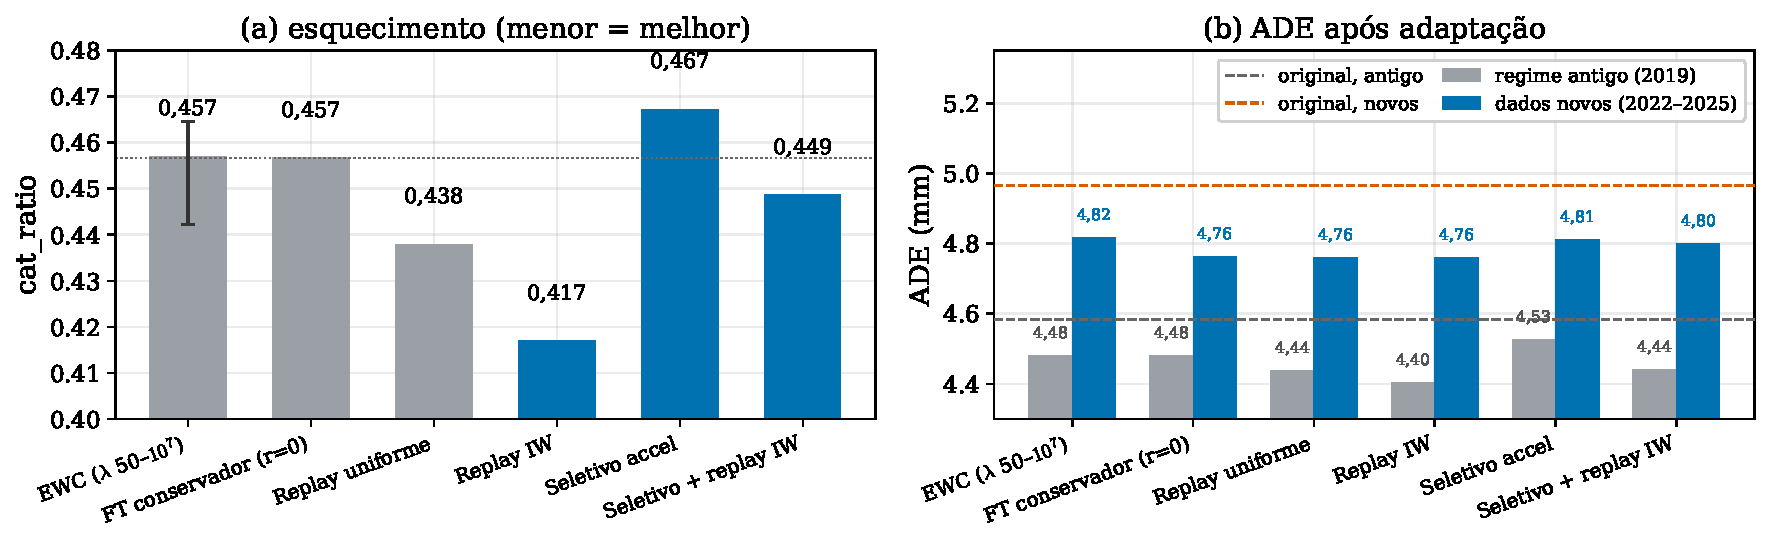
\includegraphics[width=\linewidth]{fig_finetune_pt}
    \caption{Estrat\'egias de adapta\c{c}\~ao sob o mesmo protocolo (azul =
    variantes dirigidas pelo diagn\'ostico covariate/accel). (a)~Esquecimento
    (\texttt{cat\_ratio}; barra de erro = plat\^o do sweep de $\lambda$ do
    EWC; linha pontilhada = controle sem replay). (b)~ADE ap\'os a
    adapta\c{c}\~ao nos dois regimes, com o modelo original como refer\^encia
    (linhas tracejadas). O replay lidera~--- reponderar o buffer por
    import\^ancia (replay IW) atinge o menor esquecimento~---, enquanto a
    sele\c{c}\~ao dirigida pela cauda de acelera\c{c}\~ao aumenta a
    interfer\^encia em vez de reduzi-la.}
    \label{fig:finetune}
\end{figure}

\FloatBarrier
\section{Detec\c{c}\~ao online de drift}
\label{sec:deteccao}

A camada operacional responde \`a pergunta~4 sobre o stream de 288\,k trajet\'orias (ordenado por ano, jogo e trajet\'oria). Um detector \'e avaliado pela tr\'iade padr\~ao~\cite{gama2014,lu2019}: $\mathrm{FAR}_{2019}$, alarmes por mil trajet\'orias no ano de treino, onde n\~ao h\'a drift (teto de admissibilidade $0{,}20$/1k); \emph{cobertura}, os anos de 2021--2025 com ao menos um alarme; e \emph{lat\^encia} do primeiro alarme ap\'os cada fronteira de ano. Para eliminar o vi\'es de otimizar e reportar m\'etricas no mesmo stream, a calibra\c{c}\~ao segue valida\c{c}\~ao cruzada 2-fold \emph{por jogos}: metade dos jogos de cada ano seleciona a configura\c{c}\~ao do ADWIN~\cite{adwin} em uma grade de 96 combina\c{c}\~oes,\footnote{Confian\c{c}a $\delta$, janelas m\'inima e m\'axima e \emph{cooldown}; sele\c{c}\~ao lexicogr\'afica por cobertura $\to$ FAR $\to$ raz\~ao sinal-ru\'ido.} e a outra metade, intocada pela sele\c{c}\~ao, \'e avaliada uma \'unica vez. Todos os n\'umeros s\~ao \emph{out-of-sample}, com IC de Wilson 95\,\%.

\paragraph{Detector prim\'ario (erro do modelo).}
O sinal por trajet\'oria \'e normalizado por z-robusto local (mediana/MAD em janela de 200 trajet\'orias), e essa escolha \'e a condi\c{c}\~ao de viabilidade do detector: sobre o sinal bruto, \emph{nenhuma} das 96 configura\c{c}\~oes \'e admiss\'ivel, em nenhum dos folds, e as 21 suaviza\c{c}\~oes convencionais testadas (m\'edias m\'oveis, EWMA, Holt, Savitzky--Golay) \emph{aumentam} a FAR, por introduzirem autocorrela\c{c}\~ao que viola a hip\'otese i.i.d.\ do ADWIN (Figura~\ref{fig:deteccao}a). Sobre o ADE normalizado, a fam\'ilia vencedora \'e est\'avel entre folds ($\delta\,{=}\,10^{-4}$, janelas 1\,000/5\,000): $\mathrm{FAR}_{2019}$ de $0{,}042$/1k (IC $[0{,}007;\,0{,}236]$, cobertura 5/5) no fold~A e $0{,}125$/1k ($[0{,}043;\,0{,}368]$, 4/5) no fold~B~--- 9/10 anos-fold cobertos, com lat\^encia de $0{,}2$--$1{,}5$ jogo. O protocolo importa: a configura\c{c}\~ao que a sele\c{c}\~ao \emph{in-sample} escolheria mant\'em $\mathrm{FAR}\,{\approx}\,0$, mas cobre apenas 2--3/5 anos fora da amostra~--- o holdout n\~ao apenas valida, muda a recomenda\c{c}\~ao.

\begin{figure}[t]
    \centering
    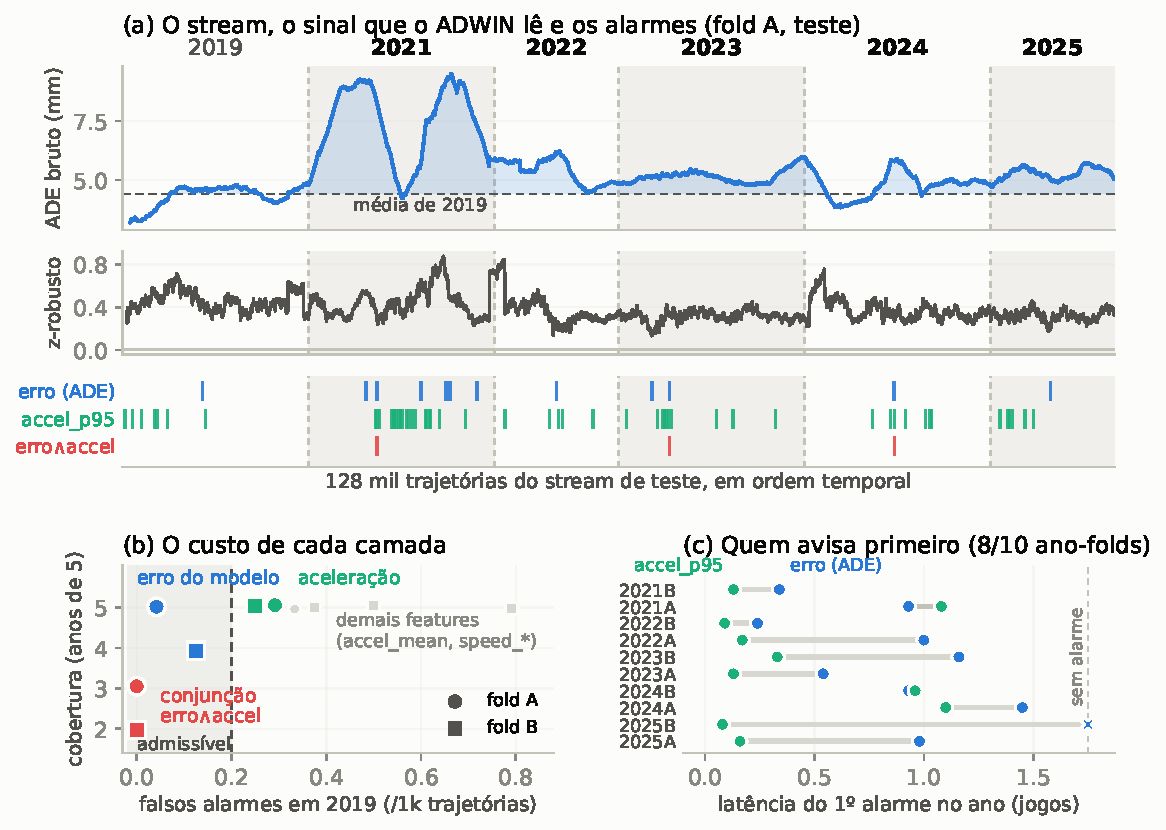
\includegraphics[width=\linewidth]{fig_deteccao_pt}
    \caption{Detec\c{c}\~ao online sob holdout 2-fold por jogos (m\'etricas no
    split de teste). (a)~O stream do fold~A: o ADE bruto sobe entre temporadas
    (topo), o z-robusto local devolve um sinal estacion\'ario~--- o que o
    ADWIN de fato l\^e (meio)~--- e o rug marca os alarmes das tr\^es camadas
    (base); em 2019 n\~ao h\'a drift, logo todo alarme ali \'e falso.
    (b)~Compromisso de cada camada: falsos alarmes contra cobertura anual;
    faixa sombreada = regi\~ao admiss\'ivel ($\leq 0{,}20$/1k); em cinza, as
    features dominadas. (c)~Lat\^encia do primeiro alarme por ano-fold: a
    acelera\c{c}\~ao antecipa o detector de erro em 8/10 casos.}
    \label{fig:deteccao}
\end{figure}

\paragraph{Vigil\^ancia dirigida pelo diagn\'ostico.}
Se o covariate shift \'e dominado pela acelera\c{c}\~ao de cauda (Tabela~\ref{tab:iw_feat}), as pr\'oprias features da janela observada~--- dispon\'iveis sem inferir o modelo e sem esperar os 15 passos futuros que o ADE exige~--- deveriam carregar o sinal de drift. O mesmo protocolo aplicado a quatro sinais cinem\'aticos confirma a previs\~ao: a admissibilidade fora da amostra reproduz o ranking da decomposi\c{c}\~ao por feature, com \texttt{accel\_p95} \`a frente ($\mathrm{FAR}\,{=}\,0{,}25$--$0{,}29$/1k, cobertura 5/5 nos dois folds) e as demais entre $0{,}29$ e $0{,}79$/1k.\footnote{Usa-se p95, e n\~ao o p99 dominante na Tabela~\ref{tab:iw_feat}, porque a janela observada cont\'em apenas 29 amostras de acelera\c{c}\~ao.} Nenhuma feature isolada \'e admiss\'ivel~--- a cinem\'atica varia naturalmente dentro de 2019~---, mas o canal de acelera\c{c}\~ao \emph{antecipa} o de erro em 8/10 anos-fold (Figura~\ref{fig:deteccao}c). No extremo oposto, a conjun\c{c}\~ao AND(ADE, \texttt{accel\_p95}) com janela de coincid\^encia $W\,{=}\,200$ zera os falsos alarmes nos dois folds (IC $[0;\,0{,}16]$/1k), ao custo de cobertura (2--3/5). O diagn\'ostico da Se\c{c}\~ao~\ref{sec:iw}, que n\~ao se converte em curadoria amostral (Se\c{c}\~ao~\ref{sec:adaptacao}), converte-se em arquitetura de monitoramento (Tabela~\ref{tab:deteccao}).

\begin{table}[t]
\centering
\caption{Arquitetura de detec\c{c}\~ao em camadas~--- m\'etricas no split de
teste (folds A/B). Todos os sinais com z-robusto $w\,{=}\,200$; configura\c{c}\~ao
de cada detector selecionada por fold na calibra\c{c}\~ao.}
\label{tab:deteccao}
\footnotesize
\begin{tabular}{llcccl}
\toprule
Camada & Sinal & FAR/1k (A/B) & Cobertura & Lat.\ (jogos) & A\c{c}\~ao \\
\midrule
Prim\'aria        & ADE seq2seq         & 0{,}042 / 0{,}125 & 5/5 / 4/5 & 0{,}2--1{,}5 & retreinar \\
Vigil\^ancia      & \texttt{accel\_p95} & 0{,}292 / 0{,}250 & 5/5 / 5/5 & 0{,}1--1{,}1 & monitorar \\
Confirma\c{c}\~ao & AND(ADE, accel)     & 0{,}000 / 0{,}000 & 3/5 / 2/5 & ---          & confirmar \\
\midrule
Corroborador      & ADE Kalman          & 0{,}167 / 0{,}083 & 5/5 / 5/5 & ---          & redund\^ancia \\
\bottomrule
\end{tabular}
\end{table}

\paragraph{Ressalvas e resultados negativos.}
A FAR por trajet\'oria assume trajet\'orias ${\sim}$i.i.d.\ em 2019, e a autocorrela\c{c}\~ao \'e real ($\rho_1\,{=}\,0{,}54$). Um teste por permuta\c{c}\~ao ($B\,{=}\,200$ sobre o bloco de 2019) mostra que a viola\c{c}\~ao \'e conservadora: embaralhar as trajet\'orias dentro dos jogos \emph{zera} os falsos alarmes em todas as r\'eplicas~--- a depend\^encia serial infla a FAR estimada, logo a admissibilidade n\~ao \'e artefato dela. Entre as alternativas, o Page-Hinkley~\cite{page_hinkley} agregado por janelas atinge $\mathrm{FAR}\,{=}\,0$, mas detecta apenas o salto de 2021 (validador de mudan\c{c}a abrupta, n\~ao monitor), e o KSWIN~\cite{kswin} \'e inadmiss\'ivel em todas as configura\c{c}\~oes ($\mathrm{FAR}\,{\geq}\,0{,}438$/1k). Por fim, um resultado negativo estrutural: conjugar detectores de \emph{escalas temporais distintas} (ADWIN por trajet\'oria $\times$ Page-Hinkley por janela) \'e invi\'avel, pois o par de alarmes mais pr\'oximo dista $\Delta_{\min}\,{=}\,214 > W$; alinhar as escalas (dois ADWIN por trajet\'oria) reduz $\Delta_{\min}$ a 3 e produz a camada de confirma\c{c}\~ao acima. A limita\c{c}\~ao \'e da combina\c{c}\~ao de escalas, n\~ao da conjun\c{c}\~ao em si.

\section{Discuss\~ao}

Os resultados respondem \`as quatro perguntas da Introdu\c{c}\~ao em cinco mensagens (pergunta 1 $\to$ mensagens 1--2; pergunta 2 $\to$ 3; pergunta 3 $\to$ 4; pergunta 4 $\to$ 5).

\textbf{1. O drift \'e real, gradual e entra pela cauda.} O ADE do seq2seq cresce nos anos p\'os-2019 (Figura~\ref{fig:degradacao})~--- em dados de composi\c{c}\~ao de liga constante (Divis\~ao A)~--- com excesso em tend\^encia crescente em 2022--2025, al\'em do salto da edi\c{c}\~ao virtual de 2021. A forma da distribui\c{c}\~ao indica que o regime novo aparece primeiro como cauda (2021) e se incorpora ao corpo do erro nos anos seguintes.

\textbf{2. O benchmark cinem\'atico degrada mais.} O aumento relativo do erro do Kalman supera o do seq2seq em praticamente todos os anos: robustez relativa maior do modelo neural, sem imunidade ao drift.

\textbf{3. O drift \'e majoritariamente covariate, dominado por acelera\c{c}\~ao de cauda.} A recovery LSIF de 59--72\,\%~--- robusta a truncamento de pesos e \`a transforma\c{c}\~ao de raz\~ao relativa, e validada pelo classifier two-sample test ($p<10^{-3}$)~--- indica que a maior parte do excesso \'e explic\'avel por covariate shift, com \texttt{accel\_p99} liderando a decomposi\c{c}\~ao por feature de forma est\'avel entre temporadas. A fra\c{c}\~ao n\~ao recuperada (${\approx}\,30$--$40\,\%$) sugere concept drift residual.

\textbf{4. O esquecimento catastr\'ofico \'e control\'avel, mas n\~ao pelo EWC.} Sob o regime antigo restrito a 2019 (2021 exclu\'ido como outlier), o \texttt{cat\_ratio} cai de 0{,}82 para 0{,}46 com ajuste conservador; o sweep de $\lambda$ em 8 ordens de grandeza mostra que a regulariza\c{c}\~ao de Fisher \'e inerte nesta arquitetura. O replay melhora esquecimento e adapta\c{c}\~ao simultaneamente, com o \'otimo no replay ponderado por import\^ancia (\texttt{cat\_ratio} 0{,}417), estabelecendo a dire\c{c}\~ao para adapta\c{c}\~ao mais profunda. J\'a a sele\c{c}\~ao \emph{dura} pela cauda de acelera\c{c}\~ao piora o esquecimento: treinar apenas na regi\~ao que mais mudou amplia a interfer\^encia, e o corpo inalterado da distribui\c{c}\~ao funciona como \^ancora. O valor do diagn\'ostico covariate est\'a no monitoramento, na explica\c{c}\~ao do excesso e na \emph{pondera\c{c}\~ao} do replay~--- n\~ao na sele\c{c}\~ao dura de amostras.

\textbf{5. Detec\c{c}\~ao operacional \'e vi\'avel na granularidade certa~--- e o diagn\'ostico vira arquitetura.} Na granularidade per-game (36 pontos), nenhum m\'etodo formal detecta; no stream per-trajet\'oria com normaliza\c{c}\~ao robusta, o ADWIN sobre o erro atinge FAR, cobertura e lat\^encia operacionais \emph{fora da amostra} (holdout por jogos)~--- e a valida\c{c}\~ao muda a recomenda\c{c}\~ao, pois a configura\c{c}\~ao selecionada in-sample n\~ao replica a cobertura. A admissibilidade dos monitores de feature reproduz o ranking do covariate shift (acelera\c{c}\~ao $>$ velocidade), o canal de acelera\c{c}\~ao antecipa o de erro em 8/10 anos-fold, e a conjun\c{c}\~ao erro$\wedge$acelera\c{c}\~ao zera os falsos alarmes observados~--- o AND s\'o \'e invi\'avel entre escalas temporais distintas.

Frente a Steuernagel e M\'aximo~\cite{seq2seq}, o avan\c{c}o est\'a em deslocar a pergunta: n\~ao \emph{se} o seq2seq supera o benchmark em um recorte fixo, mas \emph{como esse ganho evolui} quando a distribui\c{c}\~ao se afasta do treino~--- e o que fazer a respeito (adapta\c{c}\~ao e alarme operacional).

\paragraph{Limita\c{c}\~oes.}
(i)~A Divis\~ao B n\~ao est\'a representada nos dados; as conclus\~oes valem para a Divis\~ao A. (ii)~S\~ao 6 jogos por ano: os ICs por bloco s\~ao largos, a incerteza honesta da FAR (via $n_\text{eff}$) \'e maior que a nominal, e os ICs de Wilson do holdout cruzam o teto de admissibilidade~--- afirmar admissibilidade com 95\,\% de confian\c{c}a exigiria mais jogos de 2019. (iii)~O ADE \'e single-mode; modelos multimodais exigiriam min-ADE$_K$~\cite{salzmann2020,yuan2021}. (iv)~O z-robusto assume drift gradual: sob mudan\c{c}a abrupta, a normaliza\c{c}\~ao local absorveria parte do sinal. (v)~A fra\c{c}\~ao de concept drift residual n\~ao \'e isolada por feature~--- pode incluir covariate shift em features n\~ao medidas. (vi)~A edi\c{c}\~ao de 2021 foi realizada em simula\c{c}\~ao: seu salto de erro mistura a lacuna simula\c{c}\~ao--real com o drift sazonal, e as conclus\~oes de tend\^encia gradual apoiam-se em 2022--2025.

\section{Conclus\~ao}

Este artigo caracterizou, quantificou e operacionalizou o problema de data drift em um modelo seq2seq de predi\c{c}\~ao de trajet\'orias na RoboCup SSL. H\'a evid\^encia clara de degrada\c{c}\~ao temporal~--- excesso de ADE em tend\^encia crescente em 2022--2025, al\'em do salto da edi\c{c}\~ao virtual de 2021~---, maior sensibilidade do benchmark de Kalman, e drift majoritariamente covariate dominado por \texttt{accel\_p99}~--- 59--72\,\% do excesso explic\'avel por repondera\c{c}\~ao (LSIF), estimativa robusta a truncamento de pesos e \`a transforma\c{c}\~ao de raz\~ao relativa, e validada por classifier two-sample test independente.

Na resposta ao drift, duas contribui\c{c}\~oes pr\'aticas: (i)~a adapta\c{c}\~ao leve controla o esquecimento (\texttt{cat\_ratio} $0{,}82 \to 0{,}46$, com regime antigo restrito a 2019 e 2021 exclu\'ido como outlier), a regulariza\c{c}\~ao EWC \'e inerte em 8 ordens de grandeza de $\lambda$, e um buffer de replay melhora esquecimento e adapta\c{c}\~ao simultaneamente~--- com \'otimo no replay ponderado por import\^ancia (\texttt{cat\_ratio} $0{,}417$)~--- a base para adapta\c{c}\~ao mais profunda, enquanto a sele\c{c}\~ao \emph{dura} pela cauda de acelera\c{c}\~ao piora o esquecimento; (ii)~uma arquitetura de detec\c{c}\~ao em camadas validada por holdout 2-fold por jogos: detector prim\'ario sobre o erro (ADWIN + z-robusto; $\mathrm{FAR}_{2019}$ de $0{,}04$--$0{,}13$/1k fora da amostra, cobertura 9/10 anos-fold, lat\^encia $0{,}2$--$1{,}5$ jogo), canal de vigil\^ancia \emph{model-free} sobre \texttt{accel\_p95}~--- o vetor diagnosticado do drift, que antecipa o alarme de erro em 8/10 anos-fold~--- e conjun\c{c}\~ao erro$\wedge$acelera\c{c}\~ao com zero falsos alarmes observados. A taxa de falsos alarmes \'e robusta \`a depend\^encia serial do stream, e o resultado negativo do AND entre escalas temporais distintas delimita como combinar detectores em streams de erro de modelos de trajet\'oria.

\section*{Agradecimentos}
Ivan Yamasaki agradece o apoio do ITAEx e do Nubank, no \^ambito do Programa de Inicia\c{c}\~ao Cient\'ifica em Intelig\^encia Artificial do ITA (2025--2026).

\begin{thebibliography}{9}

\bibitem{seq2seq}
Steuernagel, L., M\'aximo, M. R. O. A.: Trajectory Prediction for SSL Robots Using Seq2seq Neural Networks. In: Eguchi, A., Lau, N., Paetzel-Pr\"usmann, M., Wanichanon, T. (eds.) RoboCup 2022: Robot World Cup XXV. LNCS, vol. 13561, pp. 27--38. Springer, Cham (2023). doi:10.1007/978-3-031-28469-4\_4

\bibitem{bahdanau}
Bahdanau, D., Cho, K., Bengio, Y.: Neural Machine Translation by Jointly Learning to Align and Translate. In: 3rd International Conference on Learning Representations (ICLR) (2015)

\bibitem{kalman}
Kalman, R. E.: A New Approach to Linear Filtering and Prediction Problems. Journal of Basic Engineering \textbf{82}(1), 35--45 (1960)

\bibitem{adam}
Kingma, D. P., Ba, J.: Adam: A Method for Stochastic Optimization. In: 3rd International Conference on Learning Representations (ICLR) (2015)

\bibitem{kliep}
Sugiyama, M., Nakajima, S., Kashima, H., von B\"unau, P., Kawanabe, M.: Direct importance estimation with model selection and its application to covariate shift adaptation. In: Advances in Neural Information Processing Systems (NIPS) (2008)

\bibitem{sugiyama_book}
Sugiyama, M., Kawanabe, M.: Machine Learning in Non-Stationary Environments: Introduction to Covariate Shift Adaptation. MIT Press (2012)

\bibitem{kanamori2009}
Kanamori, T., Hido, S., Sugiyama, M.: A least-squares approach to direct importance estimation. Journal of Machine Learning Research \textbf{10}, 1391--1445 (2009)

\bibitem{yamada2013}
Yamada, M., Suzuki, T., Kanamori, T., Hachiya, H., Sugiyama, M.: Relative density-ratio estimation for robust distribution comparison. Neural Computation \textbf{25}(5), 1324--1370 (2013). doi:10.1162/NECO\_a\_00442

\bibitem{lopezpaz2017}
Lopez-Paz, D., Oquab, M.: Revisiting Classifier Two-Sample Tests. In: 5th International Conference on Learning Representations (ICLR) (2017). arXiv:1610.06545

\bibitem{gama2014}
Gama, J., \v{Z}liobait\.{e}, I., Bifet, A., Pechenizkiy, M., Bouchachia, A.: A survey on concept drift adaptation. ACM Computing Surveys \textbf{46}(4), 1--37 (2014). doi:10.1145/2523813

\bibitem{lu2019}
Lu, J., Liu, A., Dong, F., Gu, F., Gama, J., Zhang, G.: Learning under concept drift: a review. IEEE Transactions on Knowledge and Data Engineering \textbf{31}(12), 2346--2363 (2019). doi:10.1109/TKDE.2018.2876857

\bibitem{adwin}
Bifet, A., Gavald\`a, R.: Learning from time-changing data with adaptive windowing. In: Proceedings of the 2007 SIAM International Conference on Data Mining (SDM), pp. 443--448 (2007). doi:10.1137/1.9781611972771.42

\bibitem{page_hinkley}
Page, E. S.: Continuous Inspection Schemes. Biometrika \textbf{41}(1--2), 100--115 (1954). doi:10.1093/biomet/41.1-2.100

\bibitem{kswin}
Raab, C., Heusinger, M., Schleif, F.-M.: Reactive Soft Prototype Computing for Concept Drift Streams. Neurocomputing \textbf{416}, 340--351 (2020). doi:10.1016/j.neucom.2020.01.119

\bibitem{kirkpatrick2017}
Kirkpatrick, J., Pascanu, R., Rabinowitz, N., et~al.: Overcoming catastrophic forgetting in neural networks. Proceedings of the National Academy of Sciences \textbf{114}(13), 3521--3526 (2017). doi:10.1073/pnas.1611835114

\bibitem{alahi2016}
Alahi, A., Goel, K., Ramanathan, V., Robicquet, A., Fei-Fei, L., Savarese, S.: Social LSTM: Human trajectory prediction in crowded spaces. In: IEEE Conference on Computer Vision and Pattern Recognition (CVPR), pp. 961--971 (2016). doi:10.1109/CVPR.2016.110

\bibitem{salzmann2020}
Salzmann, T., Ivanovic, B., Chakravarty, P., Pavone, M.: Trajectron++: Dynamically-feasible trajectory forecasting with heterogeneous data. In: European Conference on Computer Vision (ECCV) (2020). arXiv:2001.03093

\bibitem{yuan2021}
Yuan, Y., Weng, X., Ou, Y., Kitani, K.: AgentFormer: Agent-aware transformers for socio-temporal multi-agent forecasting. In: IEEE/CVF International Conference on Computer Vision (ICCV) (2021). arXiv:2103.14023

\bibitem{gu2022}
Gu, T., Chen, G., Li, J., Lin, C., Rao, Y., Zhou, J., Lu, J.: Stochastic Trajectory Prediction via Motion Indeterminacy Diffusion. In: IEEE/CVF Conference on Computer Vision and Pattern Recognition (CVPR) (2022). arXiv:2203.13777

\end{thebibliography}

\end{document}
